%++++++++++++++++++++++++++++++++++++++++
% Don't modify this section unless you know what you're doing!
\documentclass[A4,12pt]{article}
\usepackage{tabularx} % extra features for tabular environment
\usepackage{amsmath}  % improve math presentation
\usepackage{amssymb}  %load amssymb package
\usepackage{graphicx} % takes care of graphic including machinery
\usepackage[margin=1in,letterpaper]{geometry} % decreases margins
\usepackage{cite} % takes care of citations
\usepackage[final]{hyperref} % adds hyper links inside the generated pdf file
\usepackage{enumerate}
\usepackage[ddmmyyyy]{datetime}
\usepackage{caption}
\usepackage{pythonhighlight}
\usepackage[utf8x]{inputenc}
\UseRawInputEncoding

\captionsetup{font={footnotesize}}
\newtheorem{corollary}{Corollary}[section]
\hypersetup{
	colorlinks=true,       % false: boxed links; true: colored links
	linkcolor=blue,        % color of internal links
	citecolor=blue,        % color of links to bibliography
	filecolor=magenta,     % color of file links
	urlcolor=blue         
}
%++++++++++++++++++++++++++++++++++++++++


\begin{document}
\title{Supervised Learning (COMP0078) – Coursework 1}
\author{Yuan Li (18057497)\\Yuan Gao (18064382)}
\newdate{date}{10}{11}{2018}
\date{\displaydate{date}}
\maketitle

\section{PART \uppercase\expandafter{\romannumeral1}}
\subsection{Linear Regression}
\begin{enumerate}[1.]
    \item For each of the polynomial bases of dimension $k = 1, 2 , 3, 4$ fit the data set of Figure 1 \{(1,3),(2,2),(3,0),(4,5)\}.
       \begin{enumerate}[(a)]
            \item Produce a plot similar to Figure 1, superimposing the four different curves corresponding to each fit over the four data points.\\
            \textbf{Solution:} Figure \ref{fig:1a} is the four different curves corresponding to fit from dimension 1 to 4 over the four data points. \\
            \textit{Code used to implement this question can be seen in appendix. Function name: part1\_1\_1\_a().}
            \begin{figure}
              \centering 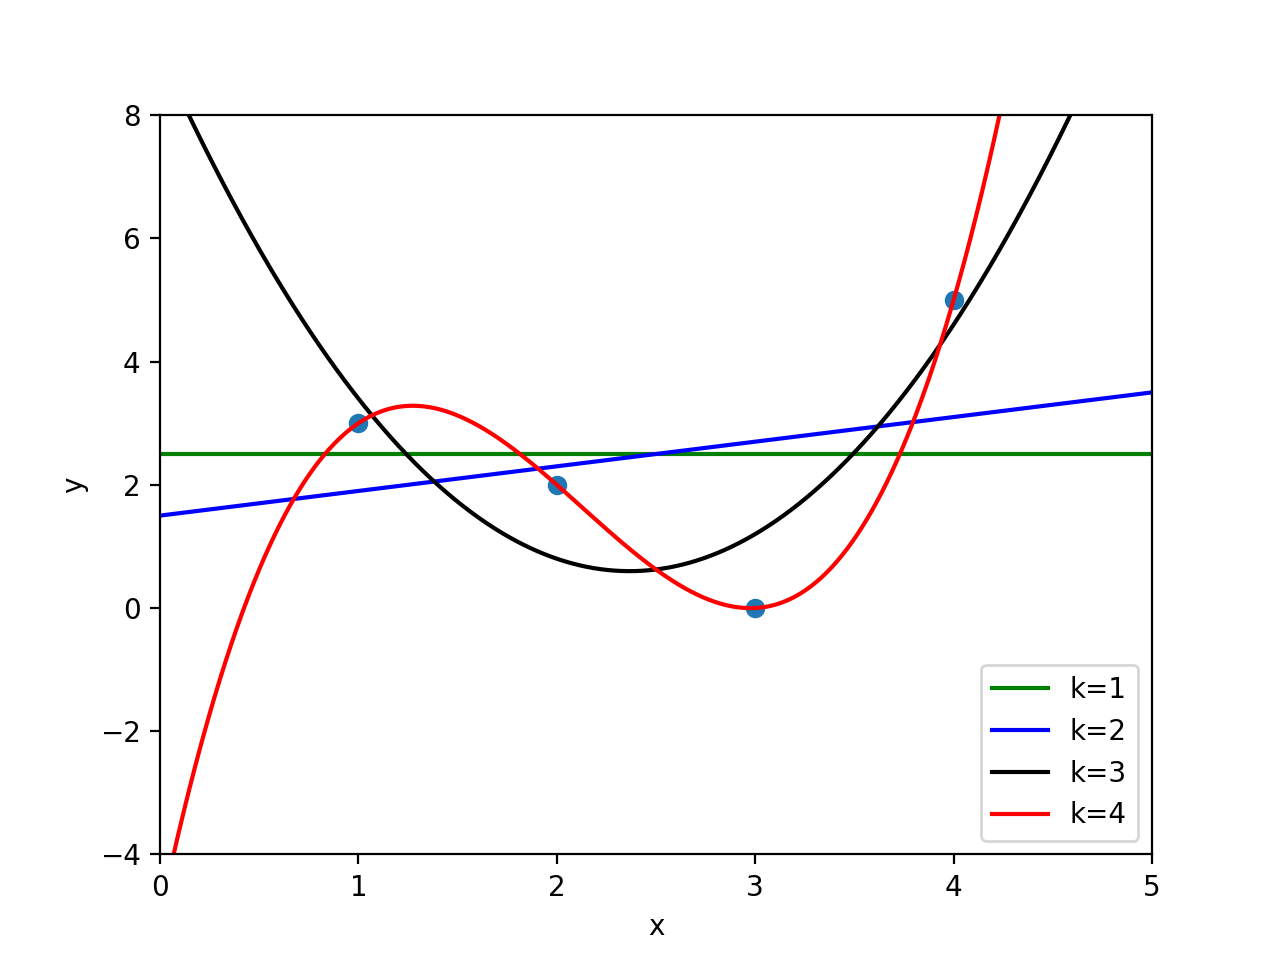
\includegraphics[width=0.8\columnwidth]{1a}
              \caption{
                \label{fig:1a}
                Curves corresponding to fit from dimension 1 to 4
              }
            \end{figure}
            \item Give the equations corresponding to the curves fitted for $k = 1, 2, 3$. The equation corresponding to $ k = 4 $ is $-5 + 15.17x - 8.5x^2 + 1.33x^3$.\\
            \textbf{Solution:} 
              \begin{itemize}
                \item when $k = 1$, $y = 2.5$,
                \item when $k = 2$, $y = 1.5 + 0.4x$
                \item when $k = 3$, $y = 9-7.1x+1.5x^2$
              \end{itemize}
            
            \item For each fitted curve $k = 1, 2, 3, 4$ give the mean square error where $MSE = \frac{SSE}{m}$\\
            \textbf{Solution:}
              \begin{itemize}
                \item when $k = 1$, MSE = 3.250000
                \item when $k = 2$, MSE = 3.050000
                \item when $k = 3$, MSE = 0.800000
                \item when $k = 4$, MSE = 0.000000
              \end{itemize}
              \textit{Code used to implement this question can be seen in appendix. Function name: part1\_1\_1\_c().}
        \end{enumerate}

    \item In this part we will illustrate the phenomena of \textit{overfitting}.
        \begin{enumerate}[(a)]
          \item 
            \begin{enumerate}[i.]
            \item Plot the function $sin^2(2\pi x)$ in the range $0 \le x \le 1$ with the points of the above data set superimposed. The plot should resemble.\\
            \textbf{Solution:} Figure \ref{fig:2a1} is the function $sin^2(2\pi x)$ in the range $0 \le x \le 1$ with the points of the above data set superimposed.\\
            \textit{Code used to implement this question can be seen in appendix. Function name: part1\_1\_2\_a\_i().}
              \begin{figure}
              \centering 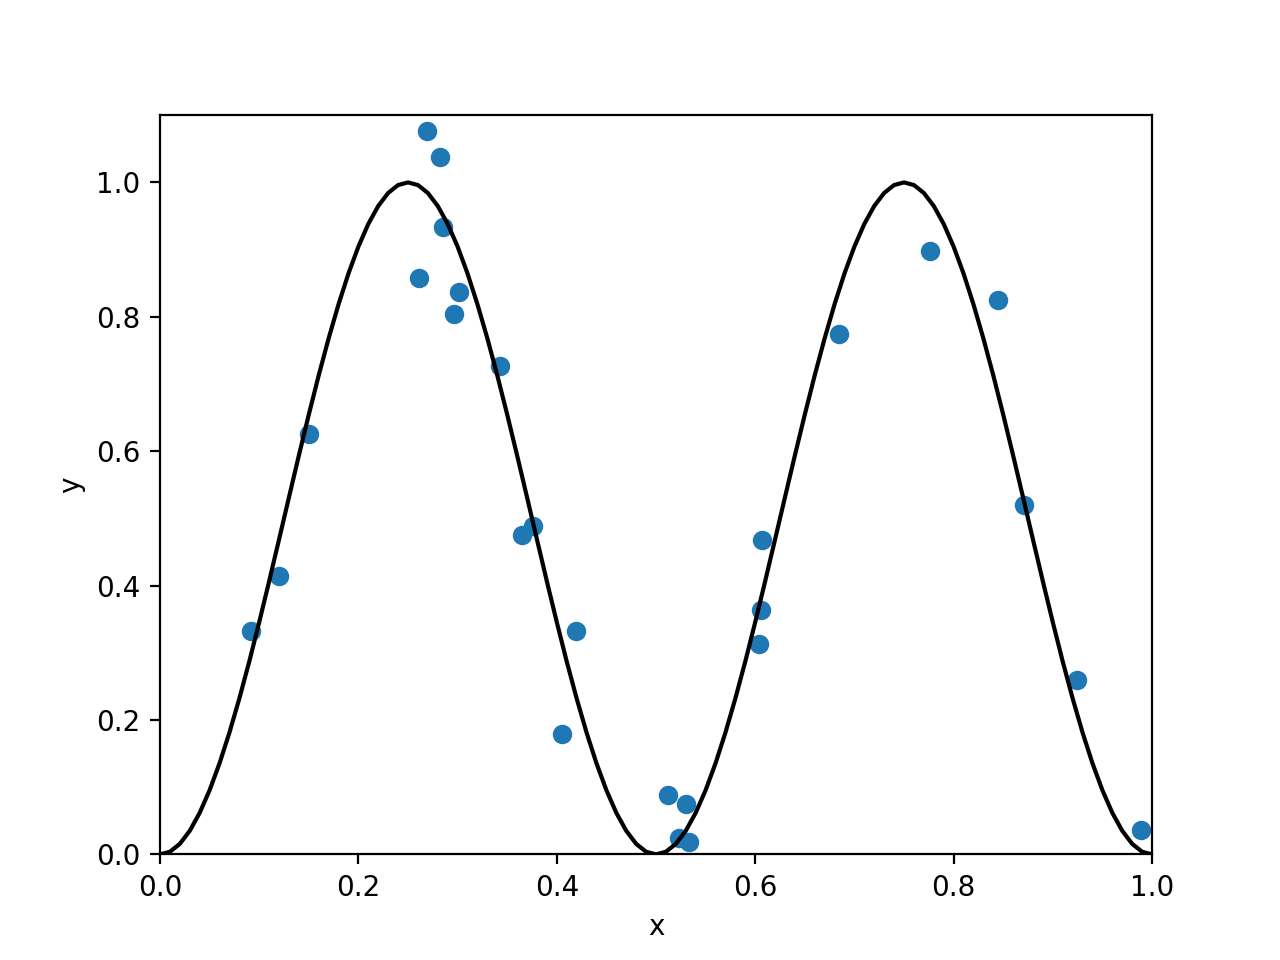
\includegraphics[width=0.8\columnwidth]{2a1}
              \caption{
                \label{fig:2a1}
                $sin^2(2\pi x)$ in the range $0 \le x \le 1$ with points within dataset
              }
              \end{figure}

            \item Fit the data set with a polynomial bases of dimension $k = 2,5,10,14,18$ plot each of these 5 curves superimposed over a plot of a data points.\\
            \textbf{Solution:} Figure \ref{fig:2a2} is curves fitted with dataset using polynomial bases of dimension $k = 2,5,10,14,18$ superimposed over a plot of data points.\\
            \textit{Code used to implement this question can be seen in appendix. Function name: part1\_1\_2\_a\_ii().}
              \begin{figure}
              \centering 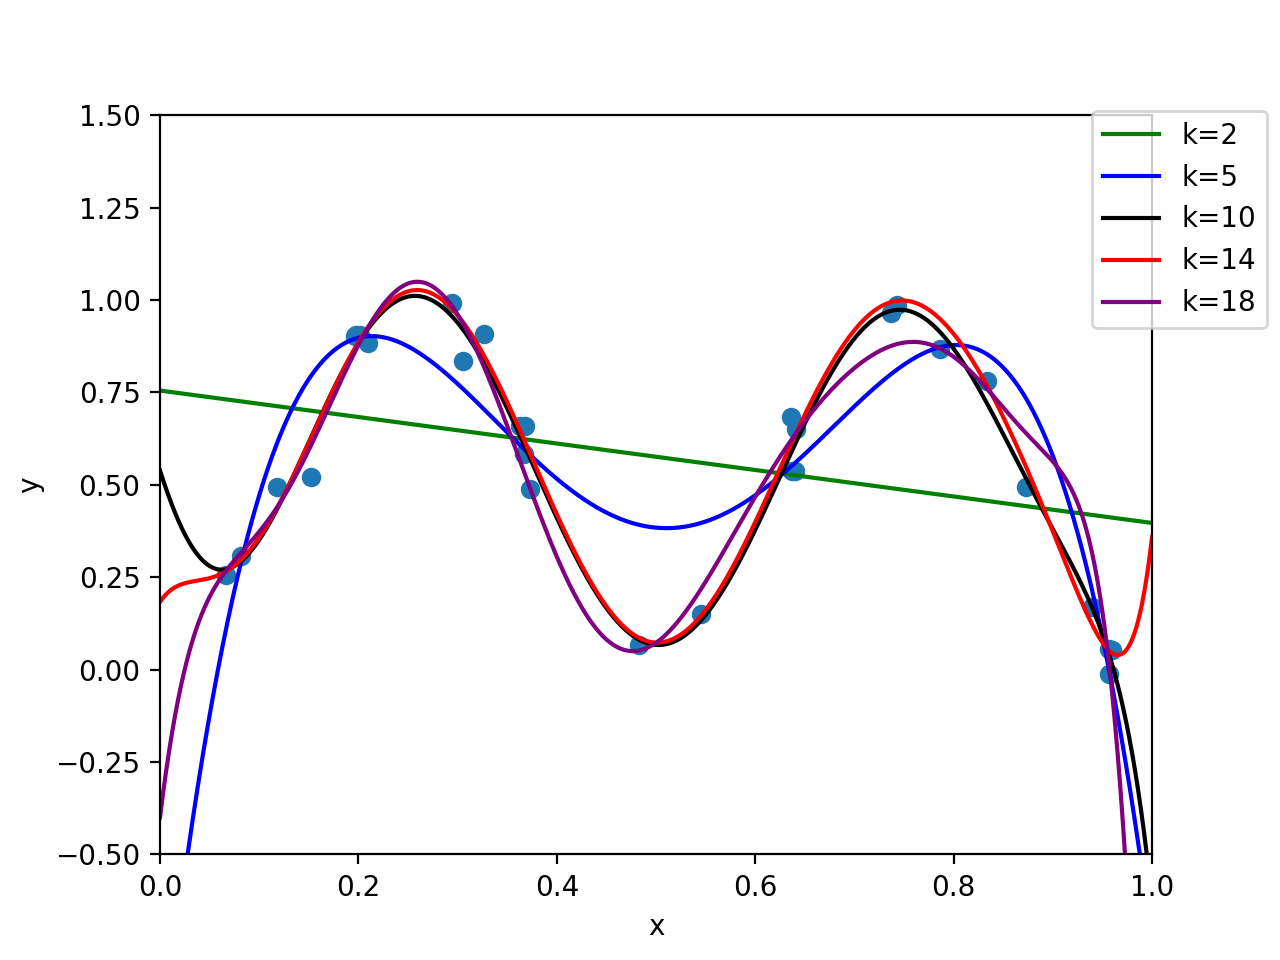
\includegraphics[width=0.8\columnwidth]{2a2}
              \caption{
                \label{fig:2a2}
                Curves with dimension $k = 2,5,10,14,18$ superimposed data points
              }
              \end{figure}
            \end{enumerate}
          \item Let the training error $te_k(S)$ denote the MSE of the fitting of the data set S with polynomial basis of dimension $k$. Plot the log of the training error versus the polynomial dimension $k = 1,...,18$(this should be a decreasing function).\\
          \textbf{Solution:} Figure \ref{fig:2b} is the plot of the log of the training error from polynomial dimension $k=1$ to $k=18$. It is a decreasing function\\
          \textit{Code used to implement this question can be seen in appendix. Function name: part1\_1\_2\_b().}
            \begin{figure}
              \centering 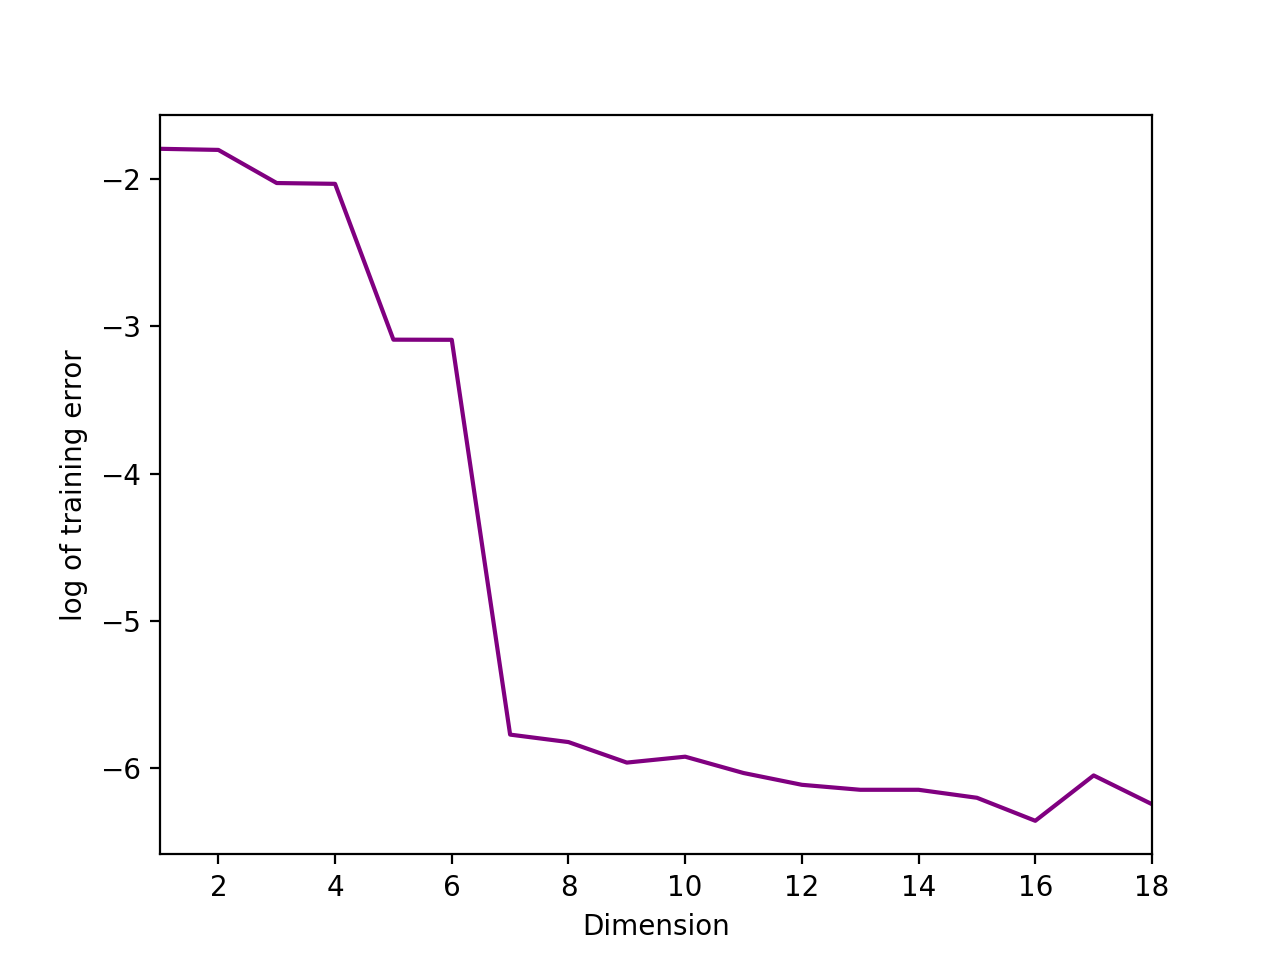
\includegraphics[width=0.8\columnwidth]{2b}
              \caption{
                \label{fig:2b}
                Log of training error from polynomial dimension $k=1$ to $k=18$
              }
              \end{figure}

          \item Generate a test set T of a thousand points,
            \begin{align}\nonumber
            T_{0.07,100} = \{(x_1,g_{0.07}(x1)),...,(x_{1000},g_{0.07}(x_{1000}))\}
            \end{align}
          Define the test error $tse_k(S,T)$ to be the MSE of the test $T$ on the polynomial of dimension $k$ fitted from training set $S$. Plot the log of the test error versus the polynomial dimension $k=1,...,18$.\\
          \textbf{Solution:} Figure \ref{fig:2c} is the plot of the log of the test error versus the polynomial dimension from $k = 1$ to $k = 18$.\\
          \textit{Code used to implement this question can be seen in appendix. Function name: part1\_1\_2\_c().}
            \begin{figure}
              \centering 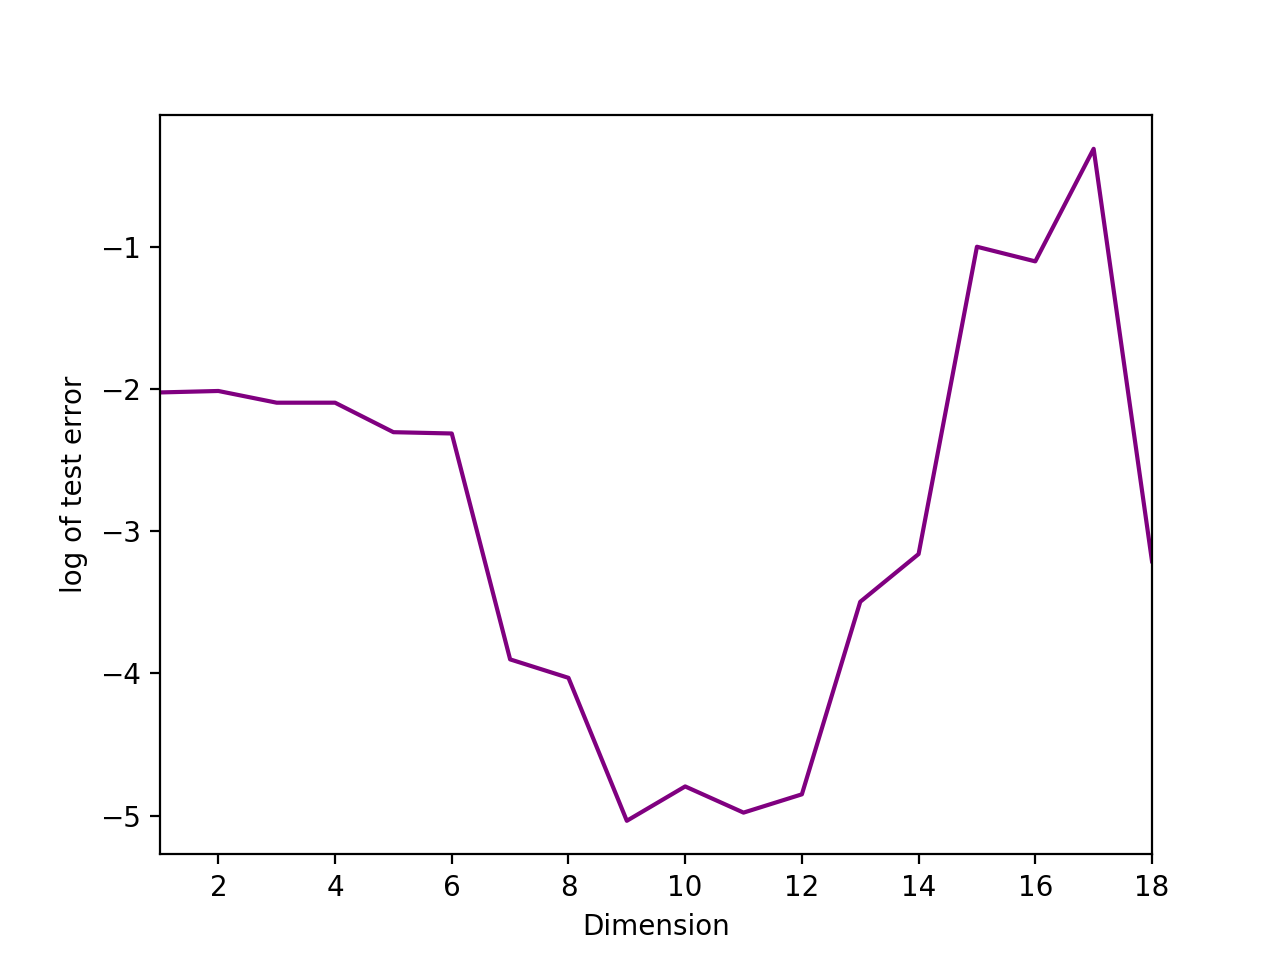
\includegraphics[width=0.8\columnwidth]{2c}
              \caption{
                \label{fig:2c}
                Log of test error from polynomial dimension $k=1$ to $k=18$
              }
            \end{figure} 
          
          \item For any given set of random numbers we will get slightly different training curves and test curves. It is instructive to see these curves smoothed out. For this part repeat items $(b)$ and $(c)$ but instead of plotting the results of a single “run” plot the average results of a 100 runs (note: plot the log(avg) rather than the avg(log)).\\
          \textbf{Solution:} After repeat items $(b)$ and $(c)$ 100 times, figure \ref{fig:2db} is the log of 100 times of average of training error and figure \ref{fig:2dc} is the log of 100 times average of testing error.\\
          \textit{Code used to implement this question can be seen in appendix. Function name: part1\_1\_2\_d().}
            \begin{figure}
              \centering 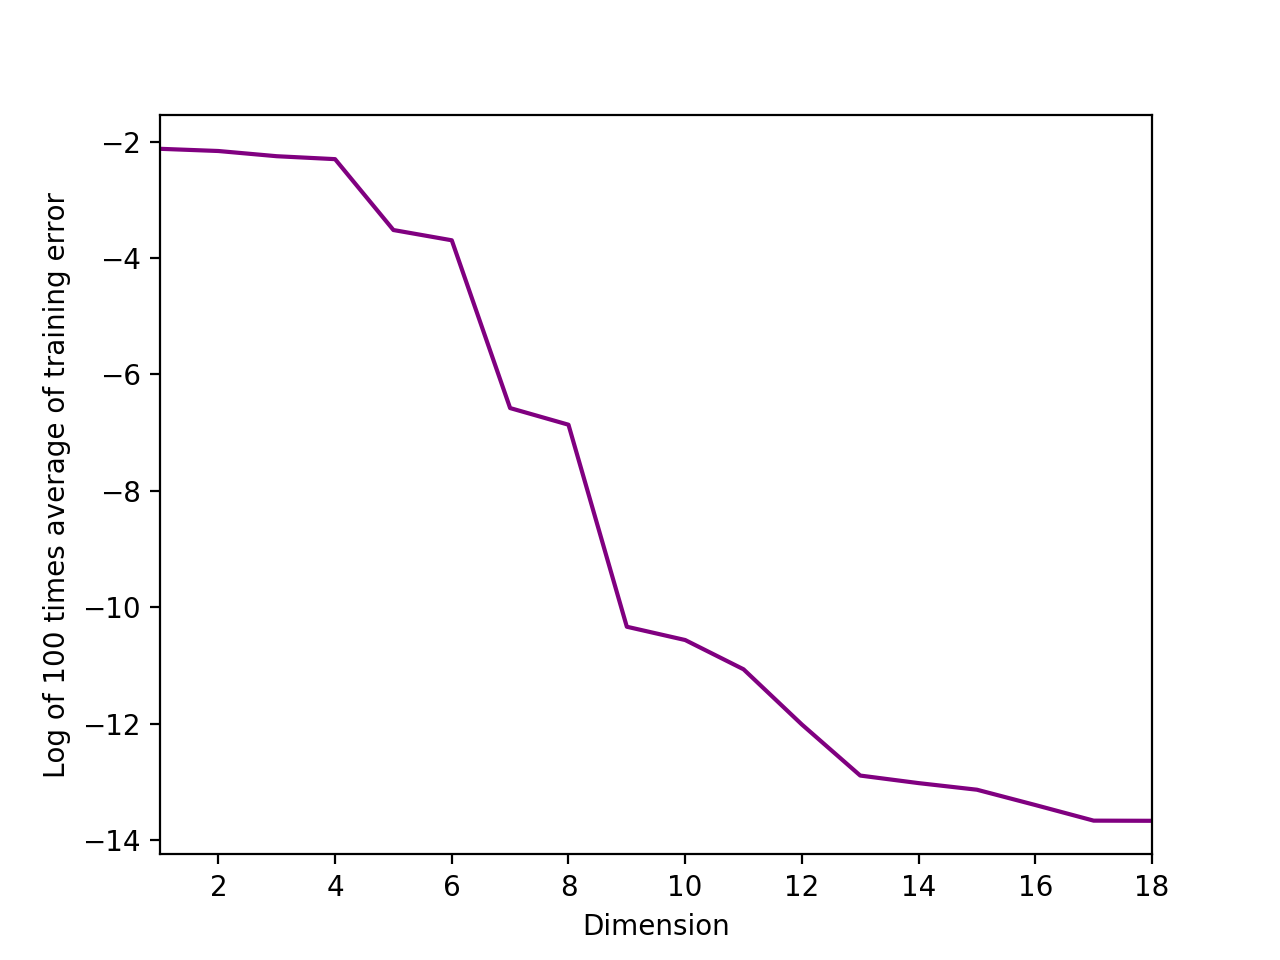
\includegraphics[width=0.8\columnwidth]{2db}
              \caption{
                \label{fig:2db}
                Log of 100 times average of training error from polynomial dimension $k=1$ to $k=18$
              }
            \end{figure}
            \begin{figure}
              \centering 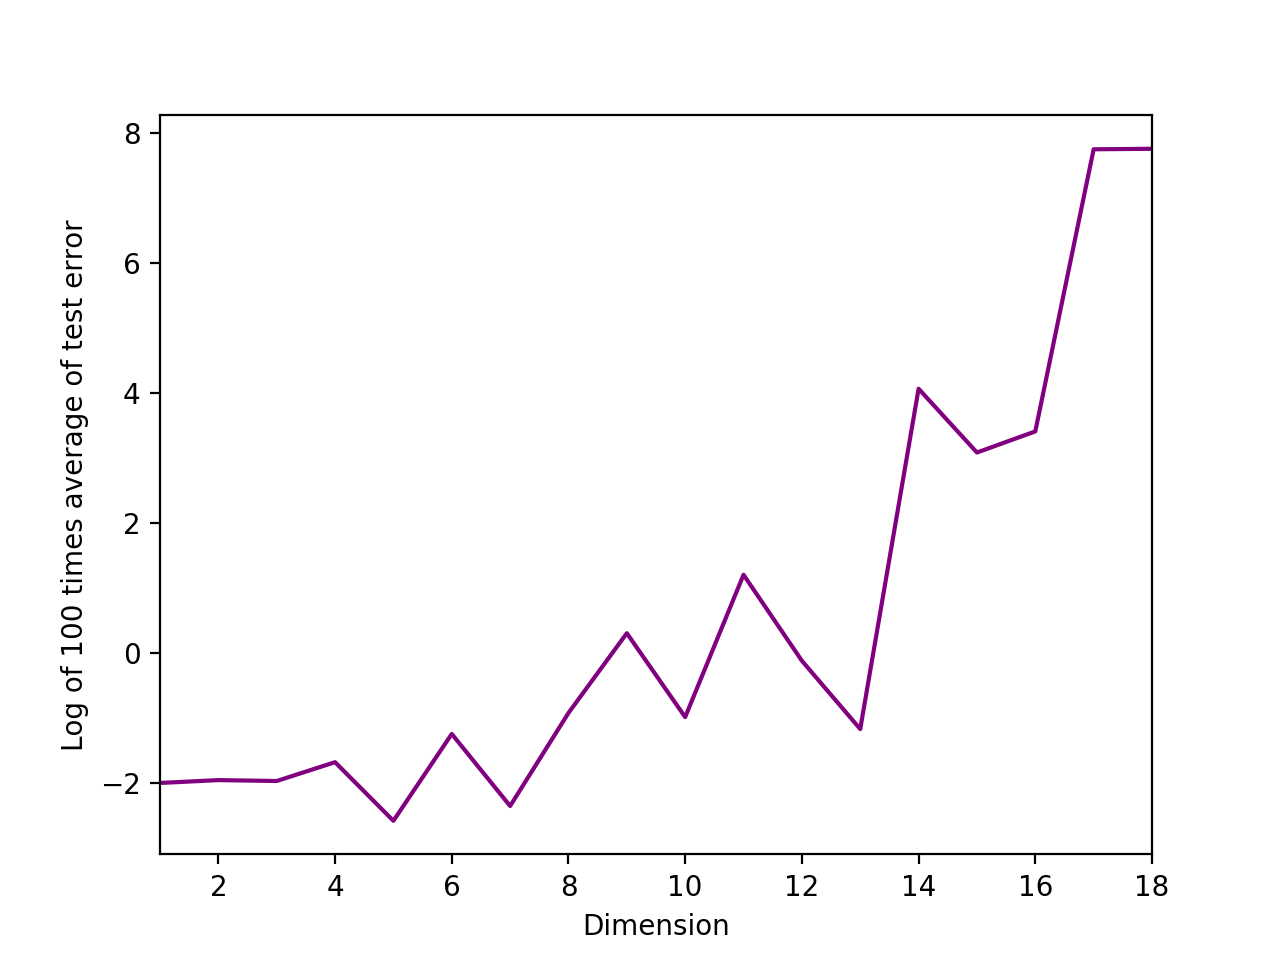
\includegraphics[width=0.8\columnwidth]{2dc}
              \caption{
                \label{fig:2dc}
                Log of 100 times average of testing error from polynomial dimension $k=1$ to $k=18$
              }
            \end{figure}
        \end{enumerate}

    \item Now use basis (for $k = 1,...,18$)
      \begin{align}\nonumber
      sin(1 \pi x), sin(2 \pi x), sin(3 \pi x),...,sin(k \pi x)
      \end{align}
    Repeat the experiments in 2 (b-d) with the above basis.\\
    \textbf{Solution:} Figure \ref{fig:3b} is the log of training error with new basis $sin(k \pi x)$. Figure \ref{fig:3c} is the log of testing error with new basis $sin(k \pi x)$. Then after repeat previous steps 100 times, figure \ref{fig:3d1} is the log of 100 times average training error and figure \ref{fig:3d2} is the log of 100 times testing error.\\
    \textit{Code used to implement this question can be seen in appendix. Function name: part1\_1\_3().}
      \begin{figure}
        \centering 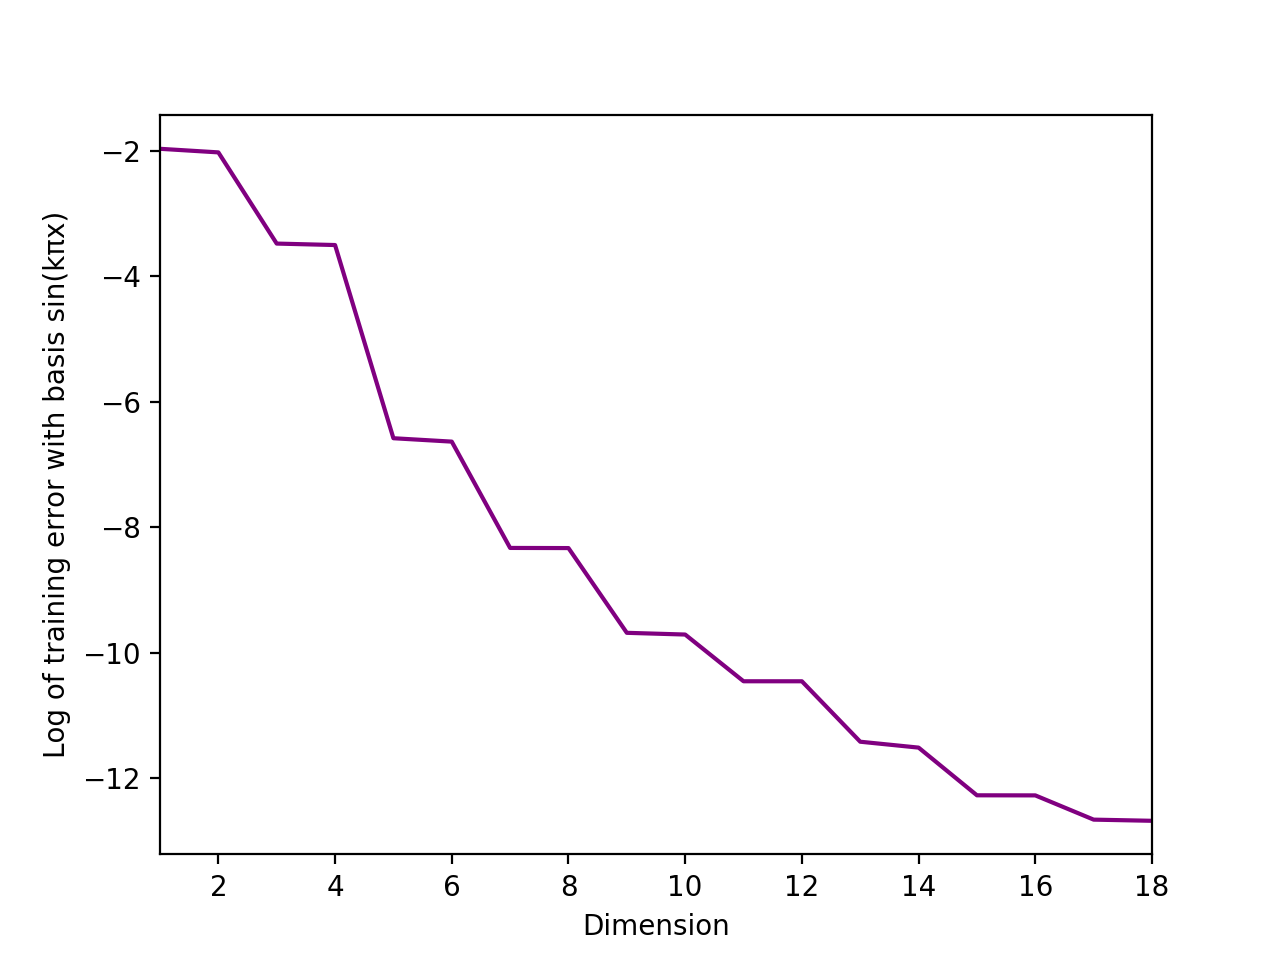
\includegraphics[width=0.8\columnwidth]{3b}
        \caption{
          \label{fig:3b}
          Log of training error with basis $sin(k \pi x)$ from dimension $k=1$ to $k=18$
        }
      \end{figure}
      \begin{figure}
        \centering 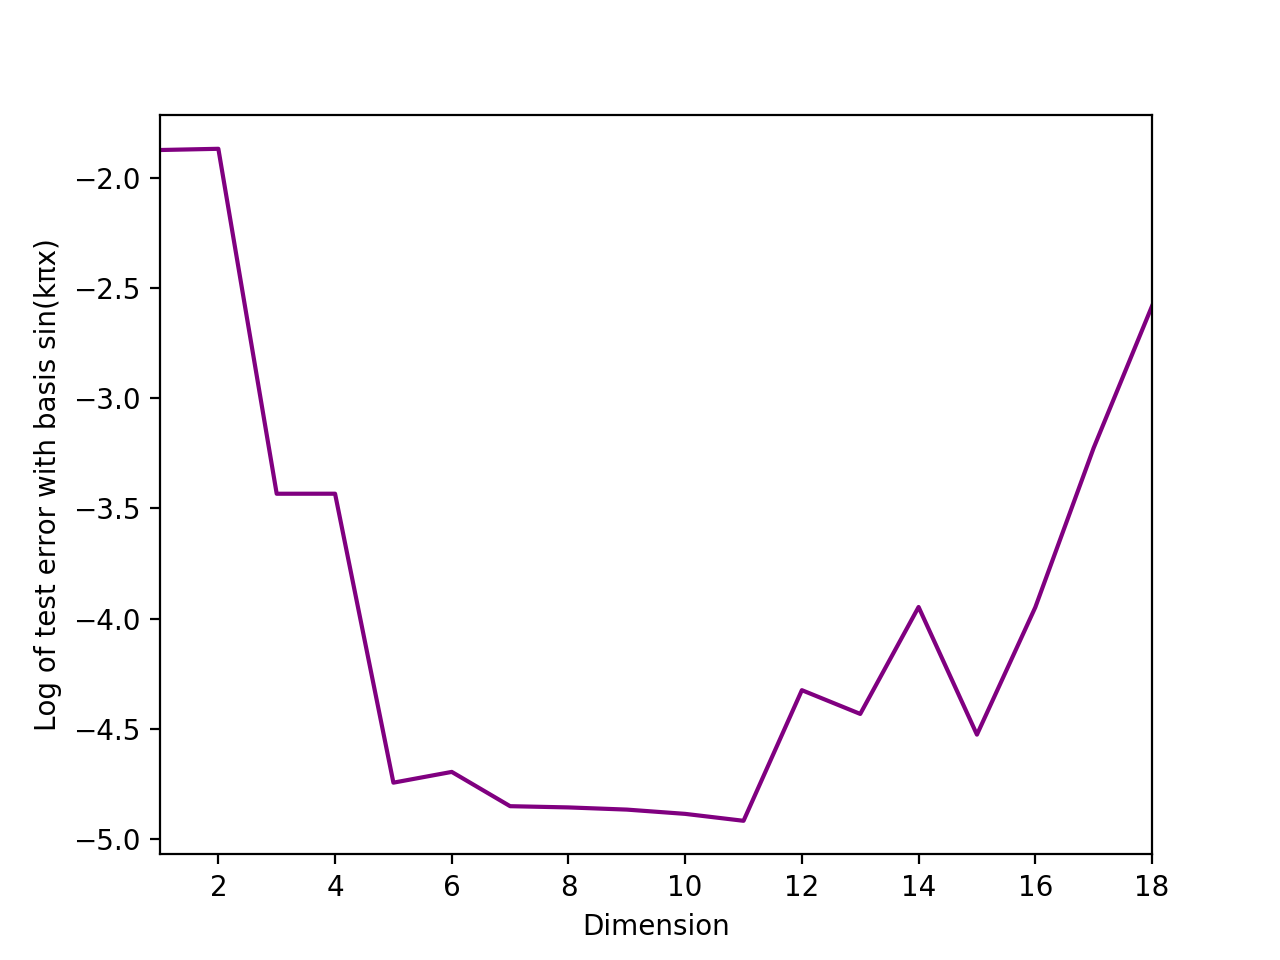
\includegraphics[width=0.8\columnwidth]{3c}
        \caption{
          \label{fig:3c}
          Log of testing error with basis $sin(k \pi x)$ from dimension $k=1$ to $k=18$
        }
      \end{figure}
      \begin{figure}
        \centering 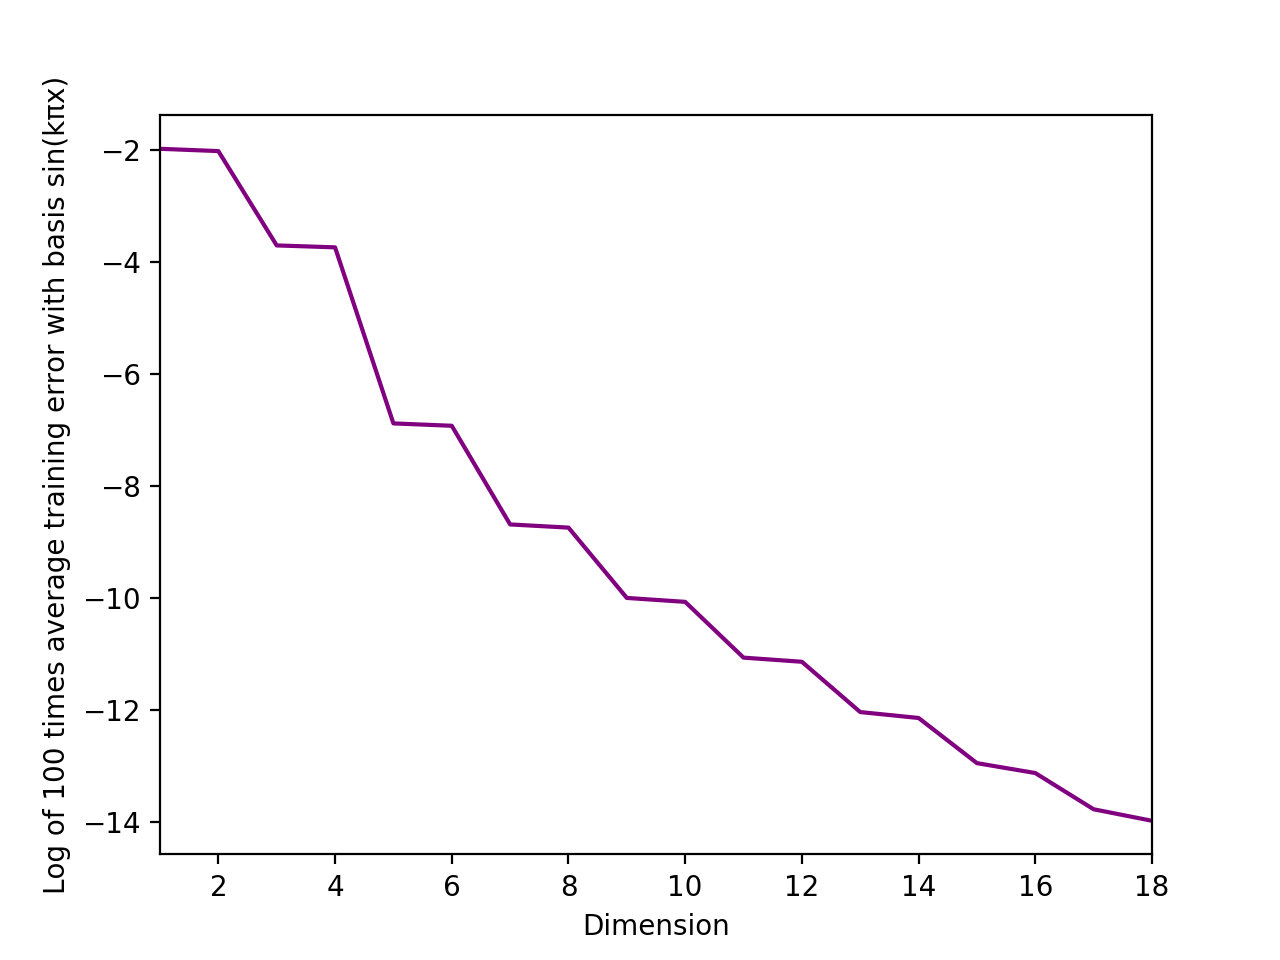
\includegraphics[width=0.8\columnwidth]{3d1}
        \caption{
          \label{fig:3d1}
          Log of 100 times average training error with basis $sin(k \pi x)$ from dimension $k=1$ to $k=18$
        }
      \end{figure}
      \begin{figure}
        \centering 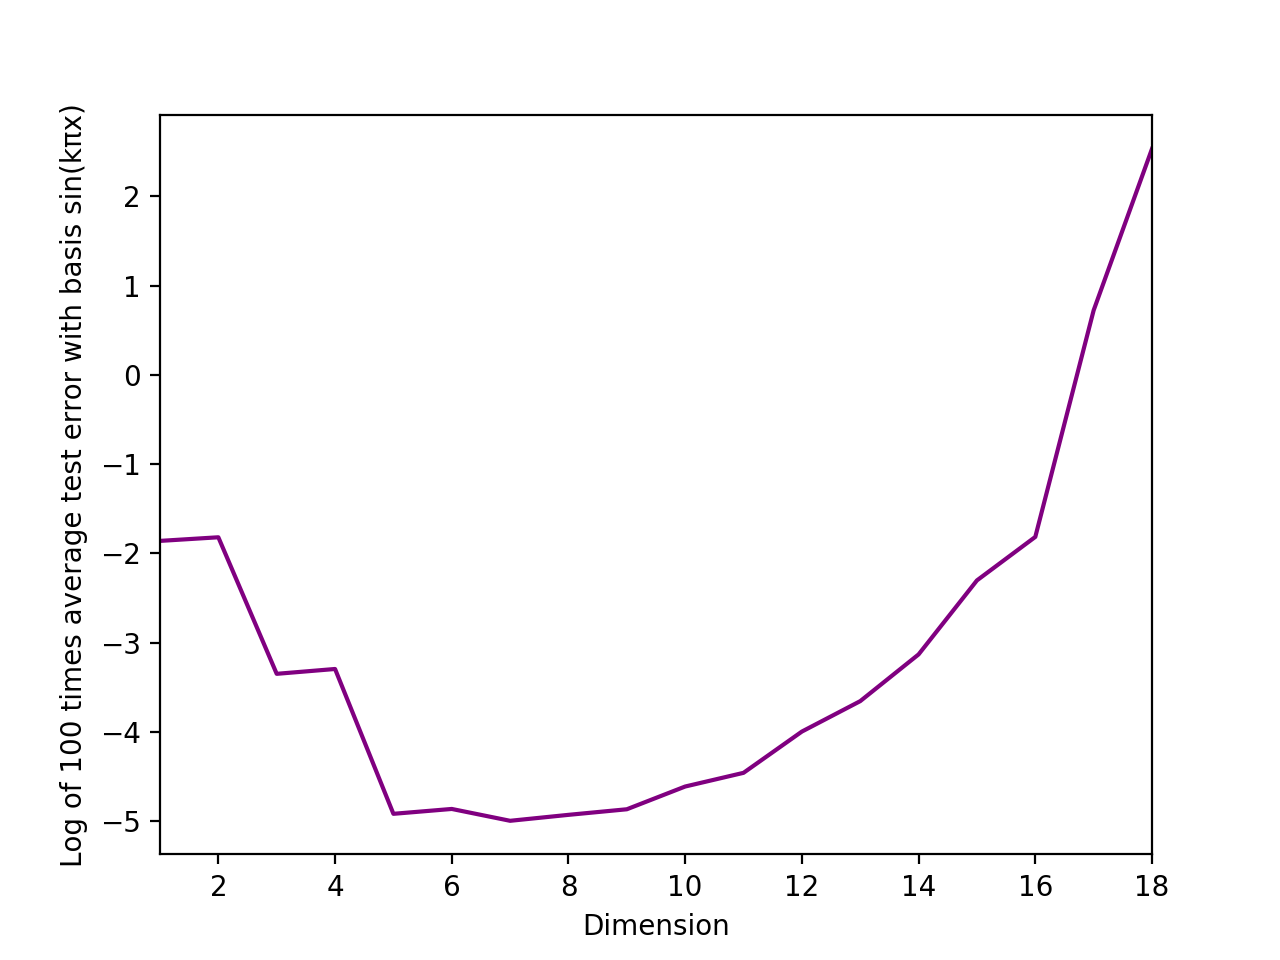
\includegraphics[width=0.8\columnwidth]{3d2}
        \caption{
          \label{fig:3d2}
          Log of 100 times average testing error with basis $sin(k \pi x)$ from dimension $k=1$ to $k=18$
        }
      \end{figure}
\end{enumerate}

\subsection{Boston housing and kernels}
\begin{enumerate}[4.]
\item 
  \begin{enumerate}[a.]
    \item Naive Regression Create a vector of ones that is the same length as the training set using the function ones. Do the same for the test set. By using these vectors we will be fitting the data with a constant function. Perform linear regression on the training set. Calculate the MSE on the training and test sets and note down the results.\\
    \textbf{Solution:}
    \begin{itemize}
      \item Average MSE on the training set is: 83.18474650412023
      \item Average MSE on the test set is: 84.90134359424864
    \end{itemize}
    \textit{Code used to implement this question can be seen in appendix. Function name: part1\_2\_a().}
    
    \item Give a simple interpretation of the constant function in ‘a.’ above.\\
    \textbf{Solution:} 
       Using constant vector $w$ to fit the data is same as calculating the average of label values. Because it just add each data all together then divided it by the number of data.

    \item Linear Regression with single attributes. For each of the thirteen attributes, perform a linear regression using only the single attribute but incorporating a bias term so that the inputs are augmented with an additional 1 entry, $(x_i , 1)$, so that we learn a weight vector $\omega \in \Re^2$ .\\
    \textbf{Solution:} 
      \begin{itemize}
        \item Linear regression attribute 1, MSE on training set: 72.30141326902927 , MSE on testing set:  69.10735255636949
        \item Linear regression attribute 2, MSE on training set: 74.0315638327025 , MSE on testing set: 71.29842498259369
        \item Linear regression attribute 3, MSE on training set: 65.45393344352883 , MSE on testing set: 62.31547619072579
        \item Linear regression attribute 4, MSE on training set: 82.30218185624605 , MSE on testing set: 79.4267323157446 
        \item Linear regression attribute 5, MSE on training set: 69.79071425404584 , MSE on testing set: 66.65809840227988 
        \item Linear regression attribute 6, MSE on training set: 43.72842548380269 , MSE on testing set: 42.65290144503359 
        \item Linear regression attribute 7, MSE on training set: 73.35922379572553 , MSE on testing set: 69.65415973232386 
        \item Linear regression attribute 8, MSE on training set: 79.92713993907894 , MSE on testing set: 76.62181525331376 
        \item Linear regression attribute 9, MSE on training set: 73.0208459509806 , MSE on testing set:  69.59720176949277 
        \item Linear regression attribute 10, MSE on training set: 66.79346452482874 , MSE on testing set: 63.3898277304275 
        \item Linear regression attribute 11, MSE on training set: 63.279843291292046 , MSE on testing set: 60.492102193894276 
        \item Linear regression attribute 12, MSE on training set: 75.66367779825535 , MSE on testing set: 72.92602617873219 
        \item Linear regression attribute 13, MSE on training set: 38.91799370292425 , MSE on testing set: 37.20829362053159
      \end{itemize}
      \textit{Code used to implement this question can be seen in appendix. Function name: part1\_2\_c().}
    \item Linear Regression using all attributes. Now we would like to perform linear regression using all of the data attributes at once.\\
    Perform linear regression on the training set using this regressor, and incorporate a bias term as above. Calculate the MSE on the training and test sets and note down the results. You should find that this method outperforms any of the individual regressors.\\
    \textbf{Solution:}
    \begin{itemize}
      \item MSE on the training set is(with all attributes): 20.77517682633871
      \item MSE on the testing set is(with all attributes): 21.109852013414205
    \end{itemize}
     \textit{Code used to implement this question can be seen in appendix. Function name: part1\_2\_d().}
  \end{enumerate}
\end{enumerate}

\subsection{Kernelised ridge regression}
\begin{enumerate}[5.]
\item
  \begin{enumerate}[a.]
    \item Create a vector of $\gamma$ values $[2^{-40}, . . . , 2^{-26}]$ and a vector of $\sigma$ values $[2^{7}, 2^{7.5}, . . . , 2^{12.5}, 2^{13}]$. Perform kernel ridge regression on the training set using five-fold cross-validation to choose among all pairing of the values of $\gamma$ and $\sigma$. Choose the indices of the $\gamma$ and $\sigma$ values that perform the best to compute the predictor that you will use to report the test and training error.\\
    \textbf{Solution:} The best $\gamma$ and $\sigma$ values we choose to report the test and training error is:
    \begin{itemize}
      \item $\gamma = 2^{-32} $
      \item $\sigma = 2^{10}$
    \end{itemize}
    \textit{Code used to implement this question and calculate best $\gamma$ and $\sigma$ values can be seen in appendix. Function name: part1\_3a()}
    
    \item Plot the “cross-validation error” (mean over folds of validation error) as a function of $\gamma$ and $\sigma$.\\
    \textbf{Solution:} Figure \ref{fig:5b1} is the plot of cross-validation error in 3 dimensional view and figure \ref{fig:5b2} is the plot of cross-validation in matrix view.\\
        \begin{figure}
        \centering 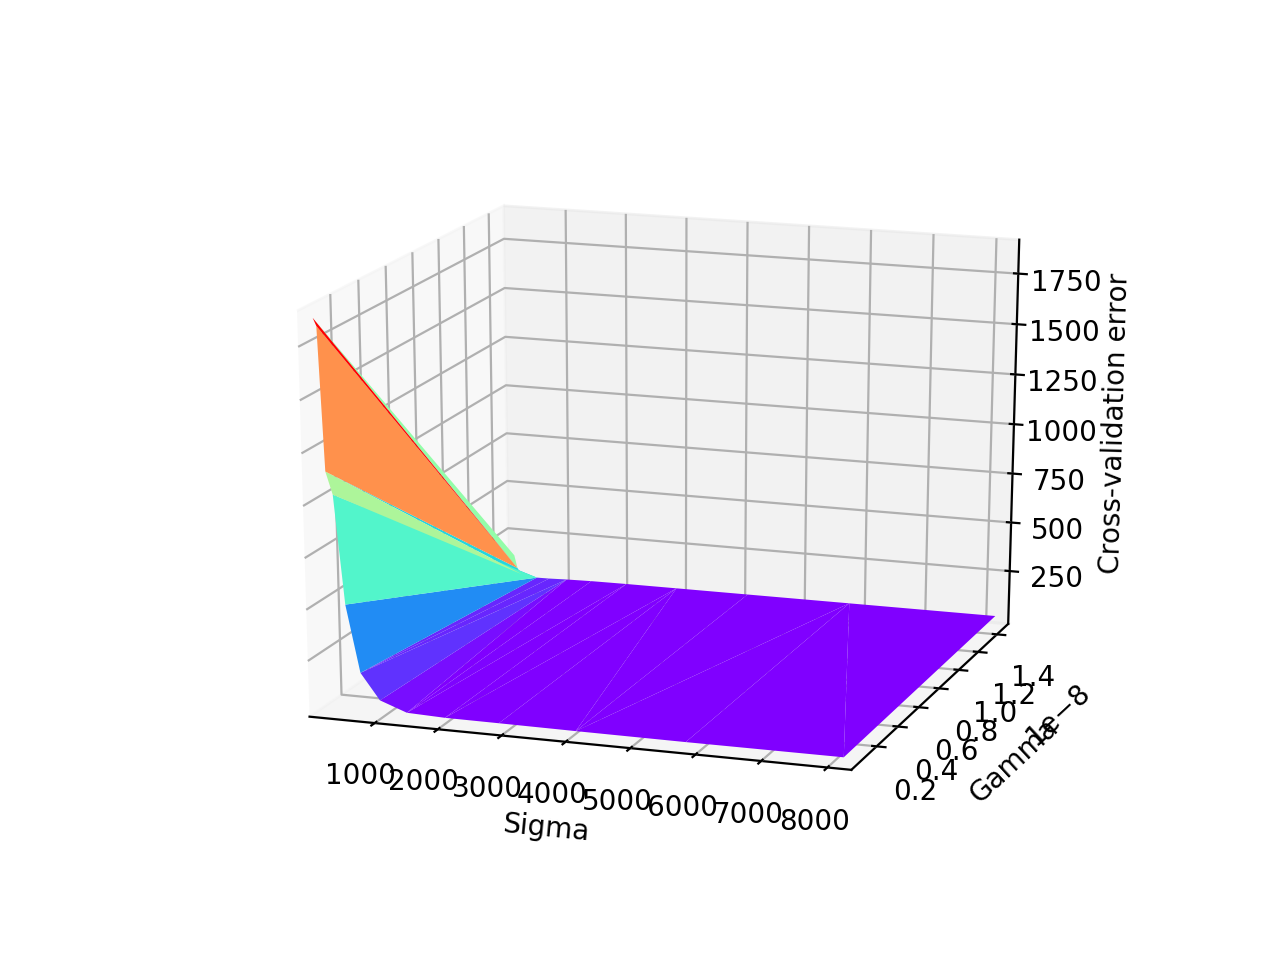
\includegraphics[width=0.8\columnwidth]{5b1}
        \caption{
          \label{fig:5b1}
          Plot of cross-validation error regarding to $\gamma$ and $\sigma$ in 3 dimension view.
        }
        \end{figure}
        \begin{figure}
        \centering 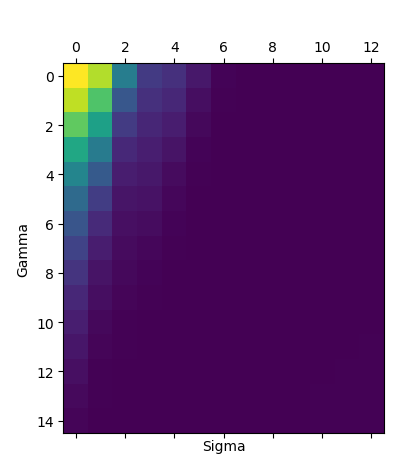
\includegraphics[width=0.8\columnwidth]{5b2}
        \caption{
          \label{fig:5b2}
          Plot of cross-validation error regarding to $\gamma$ and $\sigma$ in matrix view.
        }
        \end{figure}
    \textit{Code used to implement this question can be seen in appendix. Function name: part1\_3b()}
    
    \item Calculate the MSE on the training and test sets for the best $\gamma$ and $\sigma$.\\
    \textbf{Solution:} 
    \begin{itemize}
      \item MSE on the training set for the best $\gamma$ and $\sigma$ is: 9.413394
      \item MSE on the test set for the best $\gamma$ and $\sigma$ is: 16.937240
    \end{itemize}
    \textit{Code used to implement this question can be seen in appendix. Function name: part1\_3c().}

    \item Repeat "exercise 4a,c,d" and "exercise 5c" over 20 random (2/3, 1/3) splits of your data record the train/test error and the standard deviations of the train/test errors and summarise these results in the following type of table.\\
    \textbf{Solution:} After repeat "exercise 4a,c,d" and "exercise 5c" over 20 random (2/3, 1/3) splits of data. Table \ref{table:5d} is the table which contains the result.\\
    \textit{Code used to implement this question can be seen in appendix. Function name: part1\_3d()}
    \begin{center}
      \begin{table}
        \centering
        \begin{tabular}{ccc}  
          \hline                      
            \textbf{Method} & \textbf{MSE train}  & \textbf{MSE test}  \\
          \hline
            Naive Regression&85.51 $\pm$ 3.50 & 88.82 $\pm$ 7.22\\
            Linear Regression (attribute 1)  & 71.29 $\pm$ 4.61 & 70.77 $\pm$ 9.98 \\
            Linear Regression (attribute 2)  & 72.97 $\pm$ 4.16 & 73.32 $\pm$ 8.83 \\
            Linear Regression (attribute 3)  & 64.26 $\pm$ 4.18 & 64.77 $\pm$ 8.97 \\
            Linear Regression (attribute 4)  & 81.24 $\pm$ 4.62 & 81.73 $\pm$ 10.48 \\
            Linear Regression (attribute 5)  & 68.92 $\pm$ 4.15 & 68.54 $\pm$ 8.86 \\
            Linear Regression (attribute 6)  & 42.87 $\pm$ 4.36 & 44.24 $\pm$ 9.26 \\
            Linear Regression (attribute 7)  & 72.52 $\pm$ 4.86 & 71.49 $\pm$ 10.47 \\
            Linear Regression (attribute 8)  & 78.93 $\pm$ 4.85 & 78.63 $\pm$ 10.70 \\
            Linear Regression (attribute 9)  & 71.82 $\pm$ 4.41 & 71.87 $\pm$ 9.62 \\
            Linear Regression (attribute 10)  & 65.62 $\pm$ 4.17 & 65.58 $\pm$ 9.05 \\
            Linear Regression (attribute 11)  & 61.92 $\pm$ 3.52 & 63.14 $\pm$ 7.92 \\
            Linear Regression (attribute 12)  & 74.73 $\pm$ 3.92 & 74.81 $\pm$ 8.89 \\
            Linear Regression (attribute 13)  & 38.58 $\pm$ 2.31 & 37.79 $\pm$ 4.97 \\
            Linear Regression (all attributes)  & 21.49 $\pm$ 1.58 & 20.16 $\pm$ 3.56 \\
            Kernel Ridge Regression  & 7.78 $\pm$ 0.92 & 13.21 $\pm$ 2.81 \\
          \hline
        \end{tabular}
        \caption{Results Summary\label{table:5d}}
        \centering
      \end{table}
    \end{center}

  \end{enumerate}
\end{enumerate}

\section{PART \uppercase\expandafter{\romannumeral2}}
\subsection{Questions}
\begin{enumerate}[6.]
    \item \textit{Bayes estimator.} In the both of the following subquestions you will need to find the Bayes estimator with respect to the the probability mass function $p(x,y)$ over $(X,Y)$ where $X$ and $Y$ are finite thus $\sum_{x\in X}^{}\sum_{y\in Y}^{}p(x,y)=1$.
    \begin{enumerate}[(a)]
       \item For this subquestion $Y=[k]$ and let $c \in [0,\infty]^k$ be a vector of $k$ costs. Define $L_c : [k]\times [k] \rightarrow [0,\infty]$\\

        \textbf{Solution:}
        $Y=[k]$, $L_c(y,\hat{y})=[y\neq\hat{y}]c_y$, X and Y are $\color{red}finite$.
       We need to minimise posterior expected loss $E\left(L_c(y,\hat{y} )| X\right)$
       \begin{equation}
       \begin{aligned}
       E\left(L_c(y,\hat{y})|X\right)&=\sum_{y=1}^{k}\left[y\neq\hat{y}\right]c_y\, P(y|X=x)\\
       &= \sum_{y=1}^{k}\left[1-[y=\hat{y}]\right] c_y\,P(y|X=x)\\
       &=\sum_{y=1}^{k}c_y\,P(y|X=x)-\underset{y\in [1,k]}{[y=\hat{y}]}c_y\,P(y|X=x)
       \end{aligned}
       \end{equation}
       $\sum_{y=1}^{k}c_y\,P(y|X=x)$ is a constant, so if we want to minimise posterior expected loss, we need to maximise $[y=\hat{y}]c_y\,P(y|X=x)$

       \quad So  bayes estimator is $\hat{y}=\underset{y}{\mathrm{argmax}}\,c_y P(y|X=x)$.

       \end{enumerate}
       \begin{enumerate}[(b)]
       \item For this sub question $Y\subset\Re$. Let $L(y,\hat{y}):=|y-\hat{y}|$.Derive the Bayes estimator.\\

       \textbf{Solution:}
       $Y\subset\Re$, $\hat{y} \in \Re$, X and Y are $\color{red}finite$, $L(y,\hat{y}):=|y-\hat{y}|$
       \begin{equation}
       \begin{aligned}
       g(\hat{y})=E(L_c(y,\hat{y})\, |x)=\sum_{y\in Y}|y-\hat{y}|\, P(y|x) \quad(\hat{y}\in \Re)
       \end{aligned}
       \end{equation}
       $g(\hat{y})$ is a continuous function. So we can take derivatives. We will use the following property.
        \begin{equation}
       \begin{aligned}
       \frac{d|x|}{dx}&=\frac{d\sqrt{x^2}}{dx}=\frac{d((x^2)^\frac{1}{2})}{dx}\\
       &=\frac{1}{2} (x^2)^{-\frac{1}{2}}x=\frac{x}{|x|}
       \end{aligned}
       \end{equation}

       \begin{equation}
       \begin{aligned}
       \frac{d(g(\hat{y}))}{d\hat{y}} =\sum_{y\in Y} \frac{\hat{y}-y}{|y-\hat{y}|}P(y|x)
       \end{aligned}
       \end{equation}

       Since Y is $\color{red}finite$ set. So we rank every element in Y from smallest to largest
       $Y=[y_1,y_2 \ldots y_N]$. $\exists\; i$ such that  $Y_1 = [y_1,y_2,\ldots y_i]$ and $Y_2 = [y_{i+1},y_{i+2},\ldots y_N]$ for

       $\sum_{y\in Y_1} \frac{\hat{y}-y}{|y-\hat{y}|}P(y|x)<0$ and for
       $\sum_{y\in (Y_1\cup \{y_{i+1}\})} \frac{\hat{y}-y}{|y- \hat{y}|} P(y|x) \geqslant 0$.

       Bayes estimator is $\hat{y}=y_{i+1}$, $F(\hat{y}|X)=\frac{1}{2}$,\, $\hat{y}$ is the median of the data set $Y$.\\

       \end{enumerate}
       \begin{enumerate}[7.]
\item
\textit{Kernel modification} Consider the function $K_c(x,z):=\, c+\sum_{i=1}^{n} x_i z_i$ where $x,z\in \Re^n$.
    \begin{enumerate}[(a)]
    \item For what values of $c\in \Re$ is $K_c$ a positive semidefinite kernel? Give an argument supporting your claim.\\
    \textbf{Solution:} For $c \ge 0$ is $K_c$ a positive semidefinite kernel. Function $K_c(x,z):=\, c+\sum_{i=1}^{n} x_i z_i$ can be written as $k_c(x,z) := c+x^Tz$. For a polynomial kernel $K(x,t) = (a+x^Tt)^r$ if we let $r = 1$ then we get the same form with $K_c$. $K(x,t)$ requires $a \ge 0$, then it is sufficient to say that when $c \ge 0$, $K_c$ is a positive semidifinite kernel. \\
    In order to prove this, assume $c \ge 0$, we have to show that the kernel matrix $K_c$ should be a positive simi-defined matirx which means that for any give vector $t = [t_1,...,t_n]$, $t^{T}K_{c}t \ge 0$. \\Since:
    \begin{align}
      \begin{split}
      t^{T}K_{c}t &= \sum_{i}\sum_{j}[\mathbf{K_c}]_{ij}t_{i}t_{j}\\ 
      &= \sum_{i}\sum_{j}K_c(x_i,x_j)t_{i}t_{j}\\
      &= \sum_{i}\sum_{j}(\sum_{k=1}^{n}x_{ik}x_{jk}+c)t_{i}t_{j}\\
      &= \sum_{i}\sum_{j}(\sum_{k=1}^{n}x_{ik}x_{jk})\sum_{i}\sum_{j}t_{i}t_{j}+c\sum_{i}\sum_{j}t_{i}t_{j}\\
      &= \mathbf{K_{c}}^2||\mathbf{t}||^2+c|| \mathbf{t} ||^2\\
      &\ge 0
      \end{split}
    \end{align} 
    Since $K_c$ is positive semi-definite when $c \ge 0$, then function $K_c(x,z):=\, c+\sum_{i=1}^{n} x_i z_i$ is a positive semidifinite kernel when $c \ge 0$. 
    \end{enumerate}
    \begin{enumerate}[(b)]
    \item Suppose we use $K_c$ as a kernel function with linear regression (least squares). Explain how $c$ influences the solution.\\
    \textbf{Solution:} We use the linear regression with $K_c$ when $c \geqslant 0$. $K_c(\boldsymbol{x},\boldsymbol{z})$ is $\phi(\boldsymbol{x})$=$(x_1,\\x_2,\ldots x_l,\sqrt{c})^T$ so $K_c(\boldsymbol{x},\boldsymbol{z})$=$\phi(\boldsymbol{x})^T\phi(\boldsymbol{z})+c$ the traditional linear regression model is $y=\boldsymbol{w}^T\phi(\boldsymbol{x})$, thus, $c$ will amplification the fluctuation range of model prediction value.
    \\Regrading to this question we did some experiment in terms of different c. We use \"Boston Housing\" as our data set. Figure \ref{fig:7b1} is plot of predicted $y$ and actual $y$ within the data set when $c = 9$. Figure \ref{fig:7b2} is the plot of predicted $y$ and actual $y$ within the data set when $c = 9^7$. Figure \ref{fig:7b3} is the plot of predicted $y$ and actual $y$ within the data set when $c = 9^{15}$
    \begin{figure}[!htb]
        \centering 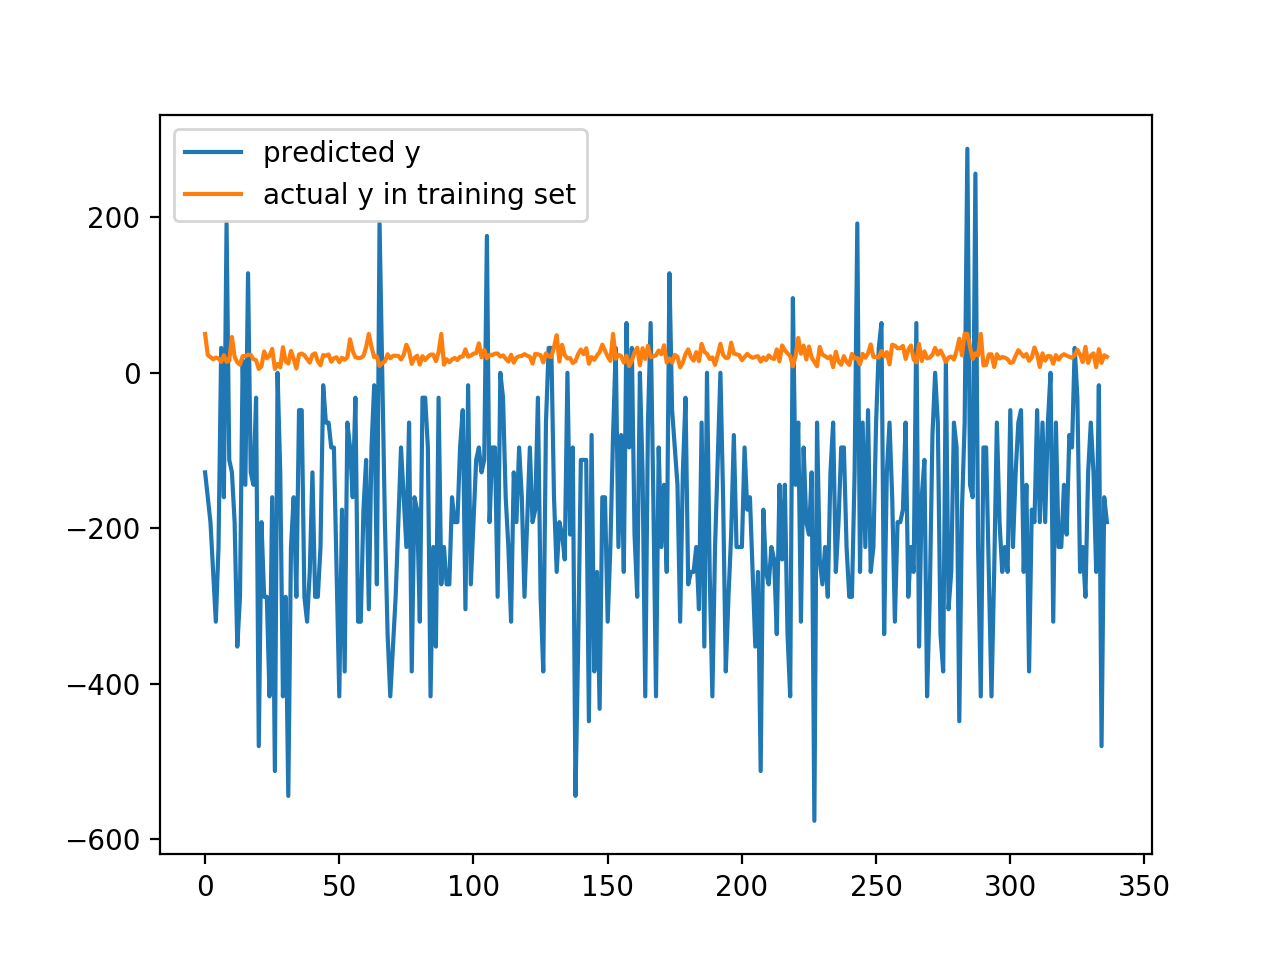
\includegraphics[width=0.8\columnwidth]{7b1}
        \caption{
          \label{fig:7b1}
          Plot of plot of predicted $y$ and actual $y$ when $c = 9$
        }
    \end{figure}[H]
    \begin{figure}[!htb]
        \centering 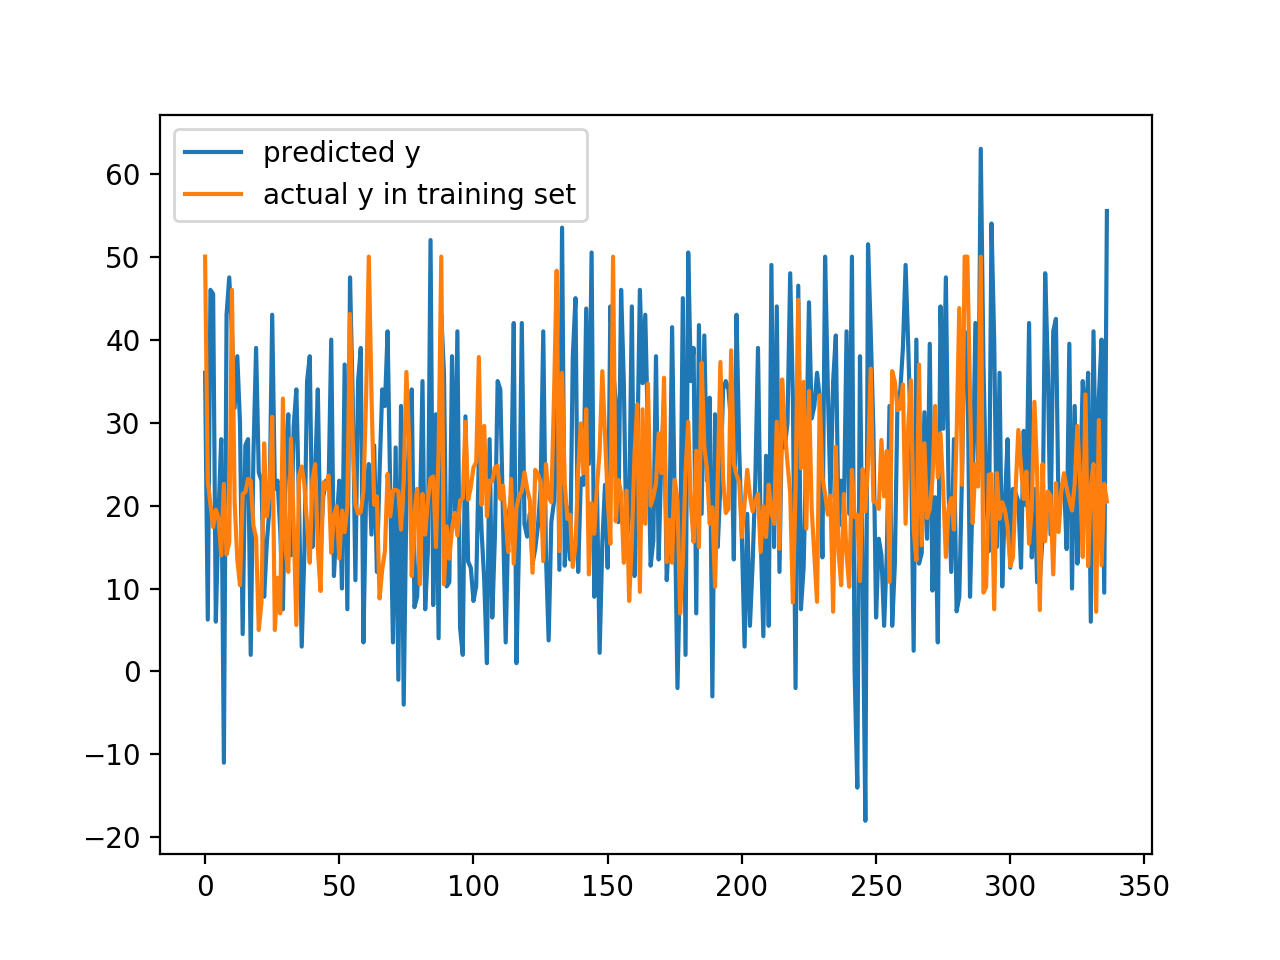
\includegraphics[width=0.8\columnwidth]{7b2}
        \caption{
          \label{fig:7b2}
          Plot of plot of predicted $y$ and actual $y$ when $c = 9^7$
        }
    \end{figure}
    \begin{figure}[!htb]
        \centering 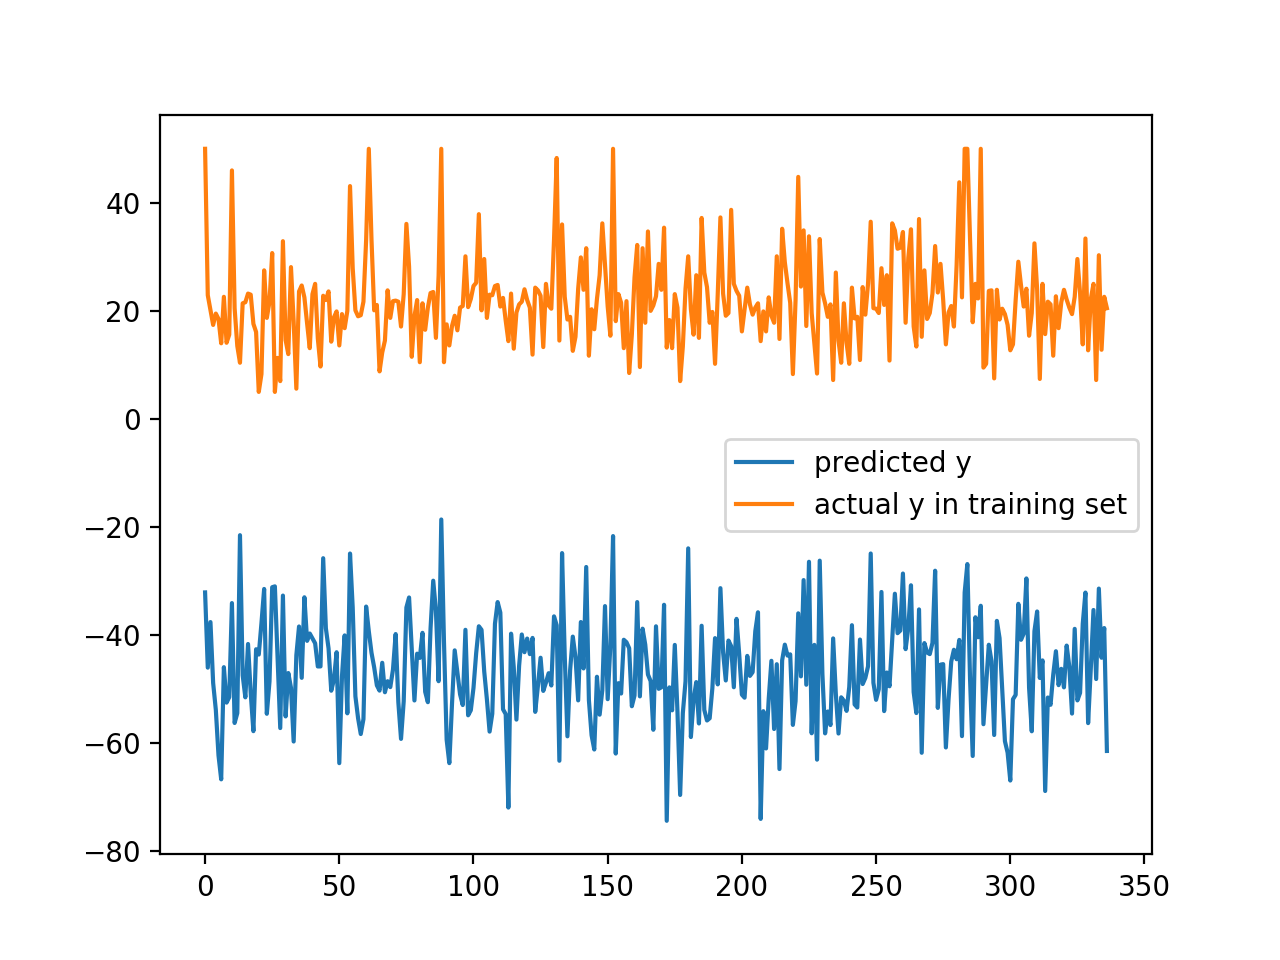
\includegraphics[width=0.8\columnwidth]{7b3}
        \caption{
          \label{fig:7b3}
          Plot of plot of predicted $y$ and actual $y$ when $c = 9^{15}$
        }
    \end{figure}
    By comparing figure \ref{fig:7b1}, \ref{fig:7b2},\ref{fig:7b3} we can conclude that $c$ can affect the fluctuation range of predicted y which will course the increasing of the MSE.  
    \end{enumerate}
\end{enumerate}
\clearpage
\begin{enumerate}[8.]
\item Suppose we perform linear regression with a Gaussian kernel $K_\beta(x,t)=exp(-\beta||x-t||^2)$ to train a classifier for two-class data (i.e., $y\in \{-1,1\})$. This classifier depends on the parameter $\beta$ selected for the kernel. How should one choose $\beta$ so that the learned linear classifier simulates a 1-$\textsc{NEAREST}\; \textsc{NEIGHBOR}\; \textsc{CLASSIFIER}$? Give an argument supporting your reasoning. \\

\textbf{Solution:} We need to simulate the 1-$\textsc{NEAREST}\; \textsc{NEIGHBOR}\; \textsc{CLASSIFIER}$ using linear regression with a Gaussian kernel. Using the kernel trick, we have $\alpha^{*}$: dual optimization formulation after kernelization which represents a linear weight vector.   and
\begin{equation}
\begin{aligned}
    K_\beta(x,t)&=exp\left(-\beta||x-t||^2\right)\\
     \alpha^{*}&=K_{\beta}^{-1} y\\
    y_{test} &= \sum_{i=1}^l \alpha^{*}_i K_{\beta}(x_i,x_{test})
\end{aligned}
\end{equation}
Since this linear classifier simulates a 1-$\textsc{NEAREST}\; \textsc{NEIGHBOR}\; \textsc{CLASSIFIER}$, we put $x_{1NN}$ in to $1NN$ algorithm as we put corresponding $x_{test}$ into linear regression with gaussian kernel. The label that assign to $x_{test}$ should be same as $y_{1NN}$.So we need to make sure:\\
$\bullet \alpha_{1NN} K(x_{1NN},x_{test})$ should have largest weight in $\sum_{i=1}^l \alpha_i K(x_i,x_{test})$.\\

In $\alpha_{1NN}K(x_{1NN},x_{test})$ which is $\alpha_{1NN}\, exp(-\beta||x_{1NN}-x_{test}||)$, the only variable we can adjust is $\beta$. \\Comparing to other term $\alpha_{others}\,exp(-\beta||x_{others}-x_{test}||)$. We focus on the ratio of exp term
\begin{equation}
\begin{aligned}
    \frac{exp(-\beta||x_{1NN}-x_{test}||)}{exp(-\beta||x_{others}-x_{test}||)}=exp\left(-\beta(||x_{1NN}-x_{test}||-||x_{others}-x_{test}||)\right)
\end{aligned}
\end{equation}

 We need to make the ratio as large as possible. So $\beta$ should be greater than zero and as large as possible theoretically.\\
$\alpha^{*}=K_{\beta}^{-1}y$ as $\beta \rightarrow \infty$ The kernel matrix will more likely to an identity matrix. Because the diagonal entries of kernel matrix will be 1 and non-diagonal entries of kernel martix will approach to 0. As $K^{-1}\rightarrow \infty$, $\alpha^{*}\rightarrow y$, $\alpha_{1NN}\rightarrow y_{1NN}$.\\
 But in practical case, when $\beta \rightarrow \infty$ it will cause underflow when calculating the $exp(-\beta\\||x_{1NN}-x_{test}||)$ So, when taking the value of $\beta$, we should take the maximum of the value that doesn't cause underflow. 


\begin{enumerate}[9.]
  \item Generalized Whack-A-Mole problem\\

  \textbf{Task}: Design an algorithm for an $n\times n$ board which, given an initial board configuration, finds a sequence of holes that you can hit in order to empty the board if such a sequence exists. The algorithm must be polynomial in n and you must provide an argument that it is correct.\\

  \textbf{Solution:} We can use matrix to express each situation on the board. For example, we are playing this game on a board with $2\times 2$ holes, $(1,2), (2,1), (2,2)$ have moles while $(1,1)$ doesn't have mole. So we can use matrix
  \[ \begin{bmatrix}
  $$
    L_3 & L_4   \\
    L_1 & L_2
  $$
  \end{bmatrix}
  \]
  And we use $L_1, L_2, L_3, L_4$ to record current state.
  $L_i$ can be $1$ or $0$.
  \begin{equation}
    \left\{
    \begin{array}{lr}
      L_1=1\\
      L_2=1\\
      L_3=0\\
      L_4=1
    \end{array}
    \right.
  \end{equation}


If this hole has mole, we assign 1 to this element, if this hole doesn't have mole, we assign 0 to this element.

    \[ \begin{bmatrix}
  0 & 1   \\
    1 & 1   \\
  \end{bmatrix}
  \]
  And we use $x_1, x_2, x_3, x_4$ to express the whack for each hole. If we whack hole 1 one time, $x_1 = 1$, similarly $x_1 = 0$ means we do nothing with hole.

operation $x_1, x_2, x_3$ can affect hole 1;\\
operation $x_1, x_2, x_4$ can affect hole 2;\\
operation $x_1, x_3, x_4$ can affect hole 3;\\
operation $x_2, x_3, x_4$ can affect hole 4;

In our algorithm, we have following theorem.

\begin{corollary}[Operation corollary]
\label{operation corollary}
For the same hole, we whack even times is equal to whack zero time; we whack odd times is equal to whack one time.
\end{corollary}

We assume at the first time, all the holes don't have any moles.
\[ \begin{bmatrix}
0 & 0   \\
  0 & 0   \\
\end{bmatrix}
\]\\
 And we do the operation $x_{1}, x_{2}, x_{3}, x_{4}$ the situation should be
\[ \begin{bmatrix}
0 & 1   \\
  1 & 1   \\
\end{bmatrix}
\]
If we do the same operation again, according to operation corollary the situation will back to the original one.

\[ \begin{bmatrix}
0 & 0   \\
  0 & 0   \\
\end{bmatrix}
\]\\
Because,we do the same operation twice, it won't change the state. In this case, $x_{1}, x_{2}, x_{3}, x_{4}$ will be our solution to this state.
\begin{equation}
  \left\{
  \begin{array}{lr}
    x_1+x_2+x_3=L_1=1\\
    x_1+x_2+x_4=L_2=1\\
    x_1+x_3+x_4=L_3=0\\
    x_2+x_3+x_4=L_4=1
  \end{array}
  \right.
\end{equation}

So we transfer this game to a solving equations problem. All the solution $x_i,  i\in n$ for $n\times n$ board is in $\{0, 1\}$.

By solving the equation above example situation, the only solution we have is:

 \begin{equation}
  \left\{
  \begin{array}{lr}
    x_1=0\\
    x_2=1\\
    x_3=0\\
    x_4=0
  \end{array}
  \right.
 \end{equation}

Which means we just need to whack hole 2, the hitting sequence is $(2)$.

For $n\times n$ board, we can consider any initial board configuration as a $n\times n$ matrix $K_n$
\[ \begin{bmatrix}
L_{n^2-n+1}   & L_{n^2-n+2}   & L_{n^2-n+3}  &\ldots     &L_{n^2}   \\
L_{n^2-2n+1} & L_{n^2-2n+2} & L_{n^2-2n+3}&\ldots     &L_{n^2-n}  \\
\vdots    & \vdots      & \vdots     &\ddots     &\vdots        \\
L_1       & L_2         & L_3        &\ldots     &L_n
\end{bmatrix}
\]\\

We use this matrix to record current state. And we have following linear equations
\begin{equation}
 \left\{
 \begin{array}{lr}
 x_1+x_2+x_{n+1}&=L_1\\
 x_1+x_3+x_{n+2}&=L_2\\
 x_2+x_4+x_{n+3}&=L_3\\
 \qquad \vdots& \\
 x_{n^2-1}+x_{n^2-n}+x_{n^2}&=L_{n^2}
 \end{array}
 \right.
\end{equation}

 So we have $n^2$ equations, we can use augmented matrix $M_a$ to express above linear equations. And the matrix only conclude coefficients is coefficient matrix $M_c$.
 \[ \left[\begin{array}{cccc|c}
 x_1   & x_2 &\ldots  & x_{n+1}       &L_1             \\
 x_1 & x_3 &\ldots& x_{n+2}    &L_2                    \\
 \vdots    & \vdots     & \vdots    &\ddots  &\vdots    \\
 x_{n^2-1} & x_{n^2-n} &\ldots & x_{n^2}& L_{n^2}
 \end{array}\right]\]
 \\

Firstly, we should calculate the rank of coefficient matrix $r_c$ and augmented matrix $r_a$. If $r_c < r_a$,  this augmented matrix has no solution which mean corresponding situation has no solution. We are solving equations in $\{0,1\}$, so the calculate rule will be slightly different especially for plus and minus:\\

$0+0=0,\, 0+1=1,\, 1+0=1,\, 1+1=0$\\
$0-0=0,\, 0-1=1,\, 1-0=1,\, 1-1=0$\\
\begin{corollary}[rank in binary domain]
\label{rank in binary domain}.\\
$(1)$ When $r_c < r_a$, linear equations have no solution.\\
$(2)$ When $r_c = r_a = n$, linear equations have unique solution.\\
$(3)$ When $r_c = r_a = k < n$, the number of solutions for linear equations is $2^{n-k}$. Because we have degree of freedom $n-k$ in binary domain.
\end{corollary}
There is no infinity solution because we are solving the problem in binary domain.
We use gaussian elimination to solve these $n^2$ equations. We perform three types of elementary row operations:\\
$\bullet$ Swapping two rows,\\
$\bullet$ Multiplying a row by a nonzero number,\\
$\bullet$ Adding a multiple of one row to another row.\\

By using above operations, we can transfer the augmented matrix into an upper triangular matrix, and in fact one that is in row echelon form. Then back substitute to get the results.\\
Here is the algorithm complexity:\\
According to gaussian elimination in  \href{https://en.wikipedia.org/wiki/Gaussian_elimination#Computational_efficiency}{
Wikipedia} it is $\mathcal{O}(n^6)$ to solve a $n^2$ equations because it requires:\\
$\bullet$ $\frac{n^2(n^2+1)}{2}$ divisions\\
$\bullet$ $\frac{2n^6+3n^4-5n^2}{6}$ multiplications\\
$\bullet$ $\frac{2n^6+3n^4-5n^2}{6}$ substractions\\

An average of $\frac{2n^6}{3}$ operations.

\end{enumerate}
\end{enumerate}
\end{enumerate}

\appendix
\clearpage
\section*{Appendix}
\subsection*{Code for linear regression}
\inputpython{linaerRegression.py}{0}{200}
\clearpage
\subsection*{Code for kernelized ridge regression}
\inputpython{KernelisedRR.py}{0}{200}
\clearpage
\subsection*{Code for main program of Part \uppercase\expandafter{\romannumeral1}}
\inputpython{CW1.py}{0}{700}
\end{document}